\chapter{The Automated Executions Plug-in}
This chapter describes the Automated Execution plug-in that is responsible for handling
the setup, control flow and display of an automated execution run.
Although the plug-in is structured according to the model-view-controller pattern this
is not the structure that this chapter will to describe it. Instead this chapter will
follow the structure already used in the previous chapters. Which means the chapter will
consist of four parts:
\begin{enumerate}
 \item The setup of an automated execution run with a description of the wizard.
 \item The input to the automated execution. This section will describe the newly created interface.
 \item The control flow of the automation with the Automation Job and the Automation Wizard.
 \item The output of the automation run. In this section the new view and the results structure will
be described.
\end{enumerate}


\section{Automation Setup - The Wizard}
\label{section:AutoWizard}
\index{Wizard}
As described in Section \ref{section:AutoConceptsSetup} an Eclipse wizard will be used to set up the 
automated run. For easy access the button for opening the wizard (

\includegraphics[scale= 0.7]{kiemAutomated.png})
is located on the tool bars of both the Execution Manager and the Automated Execution view.

The Automation Wizard consists of two pages:
\begin{enumerate}
 \item The File Selection Page for selecting all files that should be involved in the automated run.
 \item The Property Setting Page for defining custom properties that the components should receive prior to
each iteration.
\end{enumerate}


\subsection{File Selection Page}
\label{section:FileSelectionPage}
\begin{figure}[File Selection Page]
  \centering
  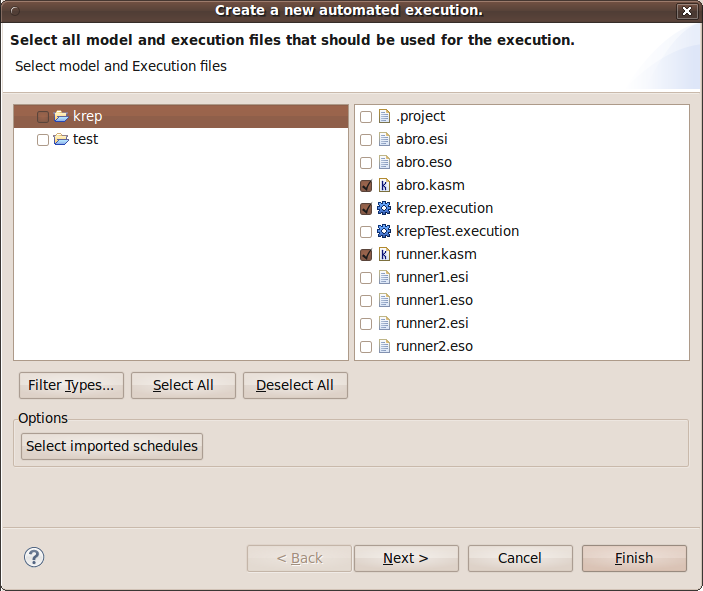
\includegraphics[scale=.4]{FileSelectionPage.png}
  \caption[The Wizard Page for selecting the input files for an automated run.]%
  {The Wizard Page for selecting the input files for an automated run.\protect}
  \label{fig:FileSelectionPage}
\end{figure}
The File Selection Page shown in Figure \ref{fig:FileSelectionPage} is used to select the model 
files and execution files that should be used for the automated run.

Since Eclipse already provides a variety of pre-made wizard pages it can be avoided to write a page for a
complex task like this from scratch. The wizard that can be modified to fit the needs of the task at hand
is the standard Eclipse Resource Import Wizard. It is normally used to select a number of files and folders
for import into the workspace. It provides a structured view where entire folders can be selected, files
can be filtered by their type and additional space is available for other buttons. In this project the files
will be 'imported' into the automated execution. This is similar enough to make it possible to use the wizard
with a few modifications and extensions.

As it should be as easy as possible to set up a run for the user it would be desirable that he doesn't need
to select all the files each time the wizard is opened. For this reason the selection will be saved into
the Eclipse preference store every time the wizard is closed. The next time the wizard is opened the selection
only has to be retrieved from the preference store and passed to the Resource Import Wizard super class.

The \ac{KIEMConfig} allows for execution files to be linked into the workspace through an extension
point. This is a useful feature for adding factory defaults and as such \ac{KIEMAuto} naturally wants to
be able to use these execution files as well. However since they these files are not in the workspace they
can't be selected through the main area of the wizard page. In order to select these files anyway a simple
list selection dialog can be accessed through the button at the bottom of the page. The dialog displays all
schedules imported through the extension point and allows the user to select any number of them.

The hard part is how to figure out if the user has selected valid files for an automated run. Recognizing selected
execution files can simply be done by looking at the file extension.
However determining whether the user selected valid model files that will work with the selected execution
files is somewhat difficult. One possibility would be to use the priority system in the \ac{KIEMConfig} in
order to determine the validity of the combinations. However this would assume that all selected execution files
are known to the plug-in and that the user set priorities for each of them. At this point it is simply assumed
that all selected files that have an extension other than 'execution' are model files. Precautions to avoid
running invalid combinations of model files and execution files are described in Section \ref{section:AutoInput}.

The dialog will only allow the user to proceed if at least one execution file or imported schedule and one
model file is selected. Otherwise an error marker will be displayed in the page header.

\subsection{Property Setting Page}
\label{section:PropertySettingPage}
\begin{figure}[Property Setting Page]
  \centering
  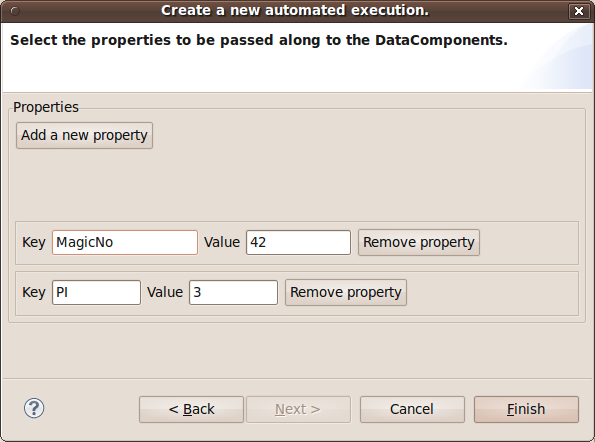
\includegraphics[scale=.4]{PropertySettingPage.png}
  \caption[The Wizard Page for setting up user defined properties.]%
  {The Wizard Page for setting up user defined properties.\protect}
  \label{fig:PropertySettingPage}
\end{figure}
The second wizard page shown in Figure \ref{fig:PropertySettingPage} allows the user to enter some custom
properties for the automated run. Unlike the first page this one doesn't extend a particular wizard page but
rather the generic wizard page that only supplies the header and the button bar at the bottom of the page.

The user can add an arbitrary number of panels for adding new (key, value) pairs through the button at the
top of the page. These values will be added to the list that is passed to all DataComponents before each iteration
and the values can be retrieved by looking for the key.

Since these properties are completely optional there are requirements for finishing this page. Which means that due
to the wizard nature of the dialog the user doesn't even have to look at that page at all but can finish directly
from the file selection page.

As with the file selection page the user input will also be stored as soon as the wizard closes and the properties
restored on the next opening of the wizard. The upside of which is that the user saves considerable work by only
having to enter the properties once. However the downside is that the user might not realize that the properties are
still set if he finishes the wizard directly from the first page. The only way to avoid this situation would be to
force the user to look at the second page. This is however very undesirable since the second page is likely to be used
only by advanced users anyway and the average user wouldn't want to see it.

\subsection{Information Processing}
\label{section:InformationProcessing}
After the user is finished with the wizard all information has to be collected in order to set up the automated run.
This involves the following steps:
\begin{enumerate}
 \item Gather the model files selected on the file selection page.
 \item Get the paths for the execution files. This might involve retrieving the paths from the schedules imported through
the extension point if the user selected any of those.
 \item Get the list of (key, value) pairs that should be added to the automated run from the second wizard page.
 \item Invoke the Automation Manager described in Section \ref{section:AutomatedRun} with the gathered parameters.
\end{enumerate}


\section{Automation Input}
\label{section:AutoInput}
In order to provide the DataComponents with input prior to each part of the automated run new interfaces
had to be created in order to interact with the components. 

\subsection{Automated Component}
An automated component is any DataComponent (see Section \ref{section:IntroDataComponent}) that wants to interact with
the automated execution plug-in. An automated component has to provide the following methods:

\begin{description}
 \item \textbf{String[] getSupportedExtensions()} :

This method is used in order to avoid the automated run encountering errors while trying to
simulate invalid combinations of model files and execution files. As soon as any execution file
is loaded the method will be called on each of the implementing classes. The classes should answer
with a list of file extensions of the model files that they can simulate. Model files that no
component in the currently active execution file can simulate will be skipped.

 \item \textbf{void setParameters(List<KiemProperty> properties) throws KiemInitializationException} : 

This method enables components to receive information prior to each execution
run. The list is implemented as an array of key, value pairs stored inside
KiemProperty objects.
At the every least the list contains the location of the model file and the
index of the currently running iteration.
This allows components to load additional files that are always in the
same path as the execution file and determine which of those to load
based on the iteration index.
The custom properties that the user defined through the wizard for example are
also added here.
If the component encounters an error during at this point because for example a model file
could not be loaded it should respond by throwing the declared Exception.

 \item \textbf{int wantsMoreSteps()} : 

This method is called before the Automation Manager performs the first step.
All components will be asked how many steps they are likely to need for their
execution run. The maximum of these values will be taken and the execution
will perform the requested number of steps. After that the components
will be asked again and so on. The process stops when all components
answer with zero.

 \item \textbf{int wantsMoreRuns()} : 

This method works analog to the wantsMoreSteps() method in the context
of entire execution runs. It is used to determine how many iterations
should be performed with the given combination of execution file and model
file.
\end{description}

\subsection{Automated Producer}
This interface extends the AutomatedComponent interface.
In addition to the inherited methods it provided one additional method.
This method is called after an iteration has finished and asks the components
if they want to publish any information about the results of their execution.
This information is gathered by the plug-in and the accumulated results
are either passed to the calling plug-in or displayed in the
specially designed view (see Section \ref{section:AutoView}).


\section{The Automated Run}
\label{section:AutomatedRun}
The Automation Manager is the key part of the automated execution. It manages the entire control flow
through the automated execution and its public methods are part of the plug-ins \ac{API}. The reason
for this is that the automated run can be initiated without the use of the wizard by any other
plug-in.

The next two sections will give a detailed description of the control flow during the automated execution.
The \ac{API} methods to initiate a new automated execution are located inside the Automation Manager. However
since those methods immediately create a new Automation Job and schedule it right away the first section will
explain the Automation Job. 

The second section will then proceed to describe the entire control flow that is managed by the Automation Manager.

\subsection{Automation Job}
\label{section:AutomationJob}
\index{Automation Job}
The Automation Job is used to run the automated execution in. As a WorkbenchJob it can execute parallel
to the normal operation of the \ac{GUI} without blocking it. It also comes with a progress monitor that
is updated by the Automation Manager through the course of the automated execution. Since an automated run
can take a very long time the user can also tell the job to run in the background while still being able
to get feedback about it through Eclipse's progress view.

Upon creation the Automation Job takes all the parameters necessary for the automated execution. After that
it opens Execution Manager view in order to load all necessary plug-ins before the actual run starts. 
The job then creates a new thread and initiates the automated execution inside the Automation Manager.
At the end it tells the calling thread that it's returning asynchronously in order not to block any callers.

The dialog showing the progress monitor is not only used to get feedback about the progress of the task
it can also be used to cancel the execution prematurely for example if the user realizes that he selected
the wrong files.

\subsection{Automation Manager}
\label{section:AutomationManager}
\index{Automation Manager}
The Automation Manager is responsible for handling the entire control flow during the automated execution.
It takes the execution files, model files and other properties as arguments and organizes the entire
run based on the available information. During the run the Automation Manager also collects the information
that will be displayed as results by the view.


- The control flow:
\begin{itemize}
 \item iterate over all execution files
 \item open execution file
 \item tell view to set up display for the first execution file
 \item iterate over all model files
 \item get first model file from list
 \item ask components how many more runs they need, take maximum and perform runs before asking again
 \item pass model file, execution file and index of iteration
 \item initialize the execution
 \item pass properties to components, at least receive model file and iteration
 \item start worker thread that listens for monitor canceling, step timing out
 \item ask components how many more steps they need, take maximum and perform steps before asking again
 \item perform one step, lock self inside semaphore, stay locked until either worker thread or event listener notifies (step done)
 \item when no component wants more steps pause
 \item gather information from all IAutomatedProducers
 \item tell view to show information for this iteration
 \item stop execution inside the KIEM and perform cleanup
 \item proceed to next iteration
 \item inform monitor of progress
 \item proceed to next model
 \item proceed to next execution
 \item when done inform monitor of done and terminate the job
\end{itemize}

\subsubsection{Modified Error Handler}
One of the problems in the early stages of development was that an automated run wouldn't complete
because of errors in some of the DataComponents.

This was caused by the fact that the Automation Manager operates only indirectly on the execution
that is running inside the Execution Manager and thus will not receive any thrown Exceptions.
Any uncaught Exception in the Execution Manager itself or in any of the DataComponents will
cause the ErrorHandler of the current Eclipse application to be invoked.

The ErrorHandler is responsible for dealing with all errors that may have to be brought
to the users attention. It contains facilities that will allow any plug-in to dispatch an
error with a predefined option of how to handle it. These options include showing the error
in the error log view, opening a dialog or opening a dialog and block the \ac{GUI} until the user
acknowledges the error. During a very long running automated run the last option is very
undesirable as it means that the automation suddenly requires user interaction which of course
defeats the whole point. This is even more annoying for the user since the majority of
Exception during an automated run that cause the \ac{GUI} to block are not critical Exceptions.

For example, one of the DataComponents is analyzing a model file with a given set of trace files.
For some reason one of the trace files is missing which causes an Exception to be thrown inside
the component which throws it to the Execution Manager that called the component. The Execution
Manager doesn't deal with the RuntimeException and throws it up to the Eclipse \ac{GUI} which
responds by invoking the ErrorHandler and blocking the automated execution from continuing. 

If the Exception could have been caught in the Automation Manager it would simply mean that
the iteration with that particular trace file would have to be skipped and the next trace file
should be used. The user then could have received the error at the end of the run or look it up
in the error log.

\listingjava
\showlistingex{code/ErrorHandlerListener.txt}
{Java}
{The interface for listeners on the ErrorHandler.}
{list:ErrorHandlerListener}
{t}
In order to remedy that situation the default ErrorHandler used by Eclipse is replaced with 
a different one. The modified ErrorHandler allows listeners that implement the interface
shown in Listing \ref{list:ErrorHandlerListener} to register to it. Whenever
a plug-in asks the ErrorHandler to deal with an error it will first notify all listeners
of the error that occurred. The listeners then can decide if they want to modify
the status of the given error. The ErrorHandler accumulates all requests from the listeners
and computes the new status. If no listeners are registered or all listeners answered
with ``Don't care'' the error will be handled with its old status. If the listeners
did request a status change all requested status changes will be applied. This
means if one listener asks to only log the error while another listener requests a pop-up
the pop-up dialog is shown and the error is logged.

However there are some errors that will be immediately handled without asking the
listeners first. Those are fatal errors that will likely cause the entire application
to enter an undefined state and where the best course of action usually is to shut down
the application entirely.

In the context of the automated execution the error handler will be asked to only log
the errors while the automated run is in progress.




\section{Automation View}
\label{section:AutoView}
- displays the information in a structured way
- start a new table for each execution file
- one row for each iteration with each model file
 - prerequisite needed here: always the same outputs throughout the entire execution file
- first columns display model file name, iteration index and current status

\subsection{Tool bar}
\label{section:AutoToolbar}
\begin{figure}[Automation View tool bar]
  \centering
  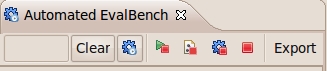
\includegraphics[scale=.8]{AutoToolbar.png}
  \caption[The tool bar in the automation view.]%
  {The tool bar in the automation view.\protect}
  \label{fig:AutoToolbar}
\end{figure}
The tool bar on the Automation View contains several actions for controlling the automated 
execution before, during and after its run (see Figure \ref{fig:AutoToolbar}).
The different controls have the following functionality (left-to-right):
\begin{enumerate}
 \item \textbf{Current Step Field} : During the automated run this field displays the
currently executing step. It is basically the same control as on the tool bar of the 
Execution Manager itself. The control was duplicated in this place in order to avoid
having to switch between the two views. This means that information about the currently
running execution is displayed in the Automation View.
 \item \textbf{Clear} : When the user initiates multiple automated runs after one another
the results are all displayed in the same view. This is the intended behavior as it should 
give the user the ability to compare automated runs with different inputs. However if the 
view gets filled with too many results the user needs an easy way to clear the view which
is realized through this button.
 \item \textbf{Automation Wizard} : The next button is used in order to launch the 
Automation Wizard. The button exists both here and on the Execution Manager's tool bar
in order to allow easy access to the automation.
 \item \textbf{Skip iteration} : During an automated run the user might realize that an
iteration has somehow locked up or isn't aborting because the components keep requesting more
steps. This button allows the user to perform a deferred termination of the current iteration
and proceed to the next index.
 \item \textbf{Skip model file} : This button has the same functionality as the one described
above but it will also skip to the next model file after aborting the current iteration. The reason
for the user wanting to cancel the current model file might be that the components keep requesting
additional runs indefinitely. Another reason would be that the model file keeps producing faulty results
due to the trace files missing and the user doesn't want to wait for it to fail on the remaining files.
 \item \textbf{Skip execution file} : Sometimes the user may even want to skip an entire execution
file if at some point it can be expected that it won't produce any useful results.
 \item \textbf{Cancel automated execution} : The last button in this group is used to initiate a deferred
termination of the entire execution. This has the same functionality as pressing ``Cancel'' inside the 
progress monitor dialog.
 \item \textbf{Export} : The export button is used for opening a dialog to export the currently displayed
results to an external format. This feature is explained in Section \ref{section:AutoExportResults}.
\end{enumerate}

\subsection{Exporting Results}
\label{section:AutoExportResults}
